\documentclass{article}
\usepackage{amsmath}  % 数学符号包
\usepackage{amssymb}  % 更多数学符号
\usepackage{enumitem} % 列表样式
\usepackage{fancyhdr} % 页眉设置
\usepackage{geometry} % 页面设置
\usepackage[UTF8]{ctex}
\usepackage{caption}
\usepackage{bm}
\usepackage{amsthm}
\usepackage{graphicx}
\everymath{\displaystyle}  % 让所有数学模式都使用 \displaystyle
\newcommand{\lb}{\left\llbracket}
\newcommand{\rb}{\right\rrbracket}
\newcommand{\np}{\noindent\par}


\geometry{a4paper, margin=1in}


\pagestyle{fancy}
\fancyhf{}
\fancyhead[C]{电子技术与系统 -- 实验累积报告}
\fancyhead[R]{2025.5}


\title{电子技术与系统 -- 实验累积报告}
\author{Noflowerzzk}
\date{2025.5}


\begin{document}
\maketitle

\section{电路基础}

\subsection{基尔霍夫电路定律}

\begin{figure}[htbp]
    \centering
    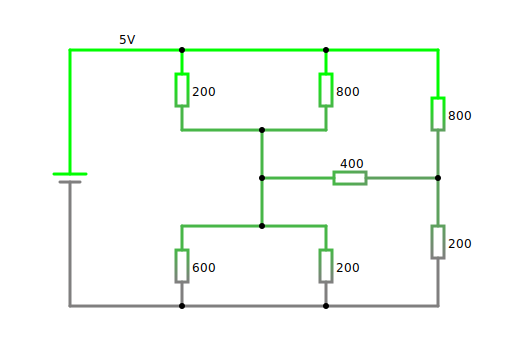
\includegraphics[width=0.5\textwidth]{KICL.pdf}
    \caption{KCL/KVL 验证}
\end{figure}

\section{晶体管输入输出特性}

\begin{figure}[htbp]
    \centering
    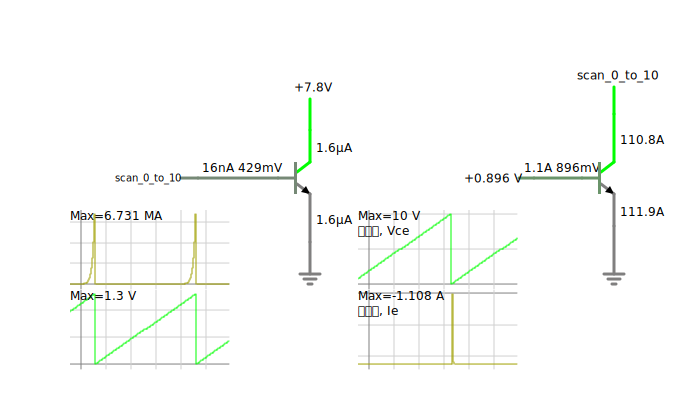
\includegraphics[width=0.7\textwidth]{晶体管输入输出.pdf}
    \caption{晶体管输入输出特性}
\end{figure}

曲线可以放大观察
\noindent \par 最大电压 $0.149 \mathrm{V}$, 也即工作区间为 $0 \mathrm{V} - 0.149 \mathrm{V}$

\section{基本放大电路}

\begin{figure}[htbp]
    \centering
    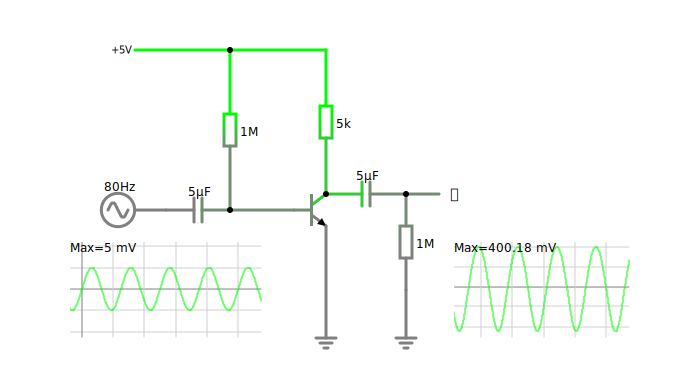
\includegraphics[width=0.7\textwidth]{基本放大电路.pdf}
    \caption{基本放大电路}
\end{figure}

$r_{be} = \frac{\beta V_E}{I_C} = 1.25 \mathrm{k}\Omega$ \np

\begin{figure}[htbp]
    \centering
    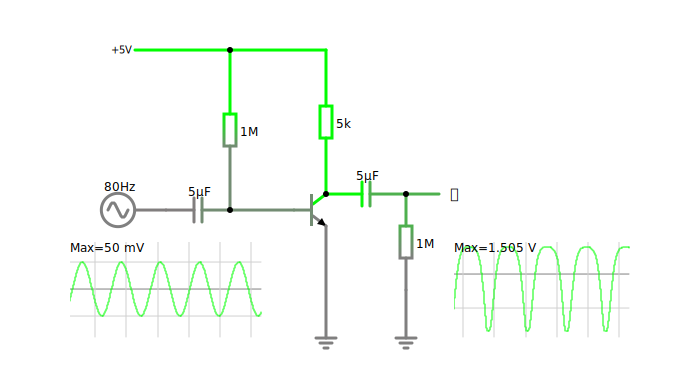
\includegraphics[width=0.7\textwidth]{基本放大电路_失真.pdf}
    \caption{基本放大电路 -- 失真}
\end{figure}

更改输入为频率80Hz、幅值50mV的交流源时,波形出现明显失真。 \np
修改方案:在发射极与地之间接入一个 $1\mathrm{k}\Omega$ 的电阻,此时输入电阻约为 $2.5 \mathrm{k}\Omega$, 放大倍数约为 $-38.5$.

\section{理想运算放大电路}

电路如图\ref{fig:yunsuanfangdaqi}
\begin{figure}
    \centering
    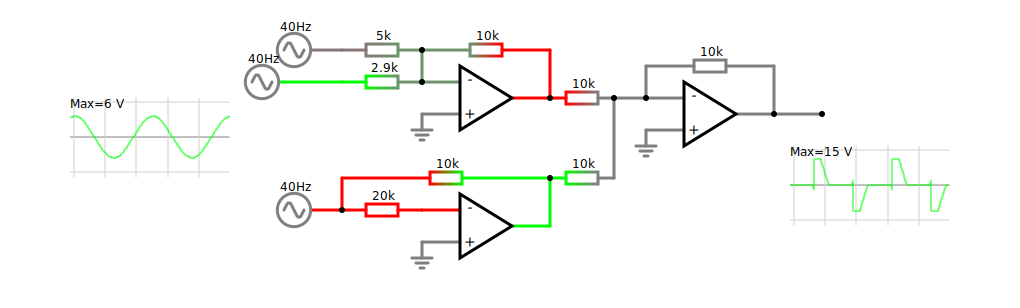
\includegraphics[width=0.9\textwidth]{运算放大器.pdf}
    \caption{运算放大器电路}
    \label{fig:yunsuanfangdaqi}
\end{figure}

三个输入信号如下:
\[
\begin{aligned}
a(t) &= \sin(\omega t) \\
b(t) &= \cos(\omega t) \\
c(t) &= -\cos(\omega t)
\end{aligned}
\]

输出波形可表示为:
\[
y(t) = 4.47 \cdot \sin(\omega t + 26.6^\circ)
\]


\section{CMOS 与非门电路}

\begin{figure}[htbp]
    \centering
    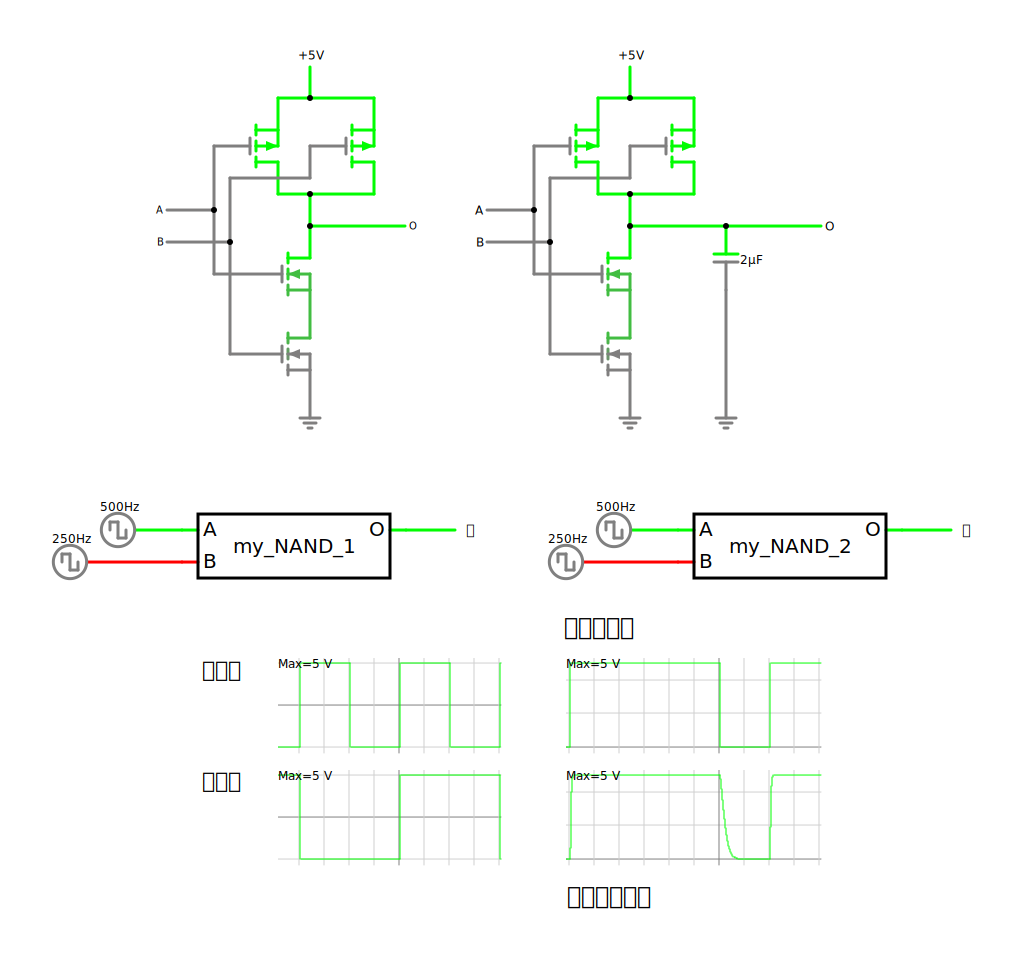
\includegraphics[width=0.7\textwidth]{NAND.pdf}
    \caption{CMOS 与非门电路}
\end{figure}

延迟测量: $t_{HL} = 0.45 \mathrm{ms}$, $t_{LH} = 0.10 \mathrm{ms}$

\section{半加器与全加器}

内容见图\ref{fig:banjiaqiyuquanjiaqi}

\begin{figure}[htbp]
    \centering
    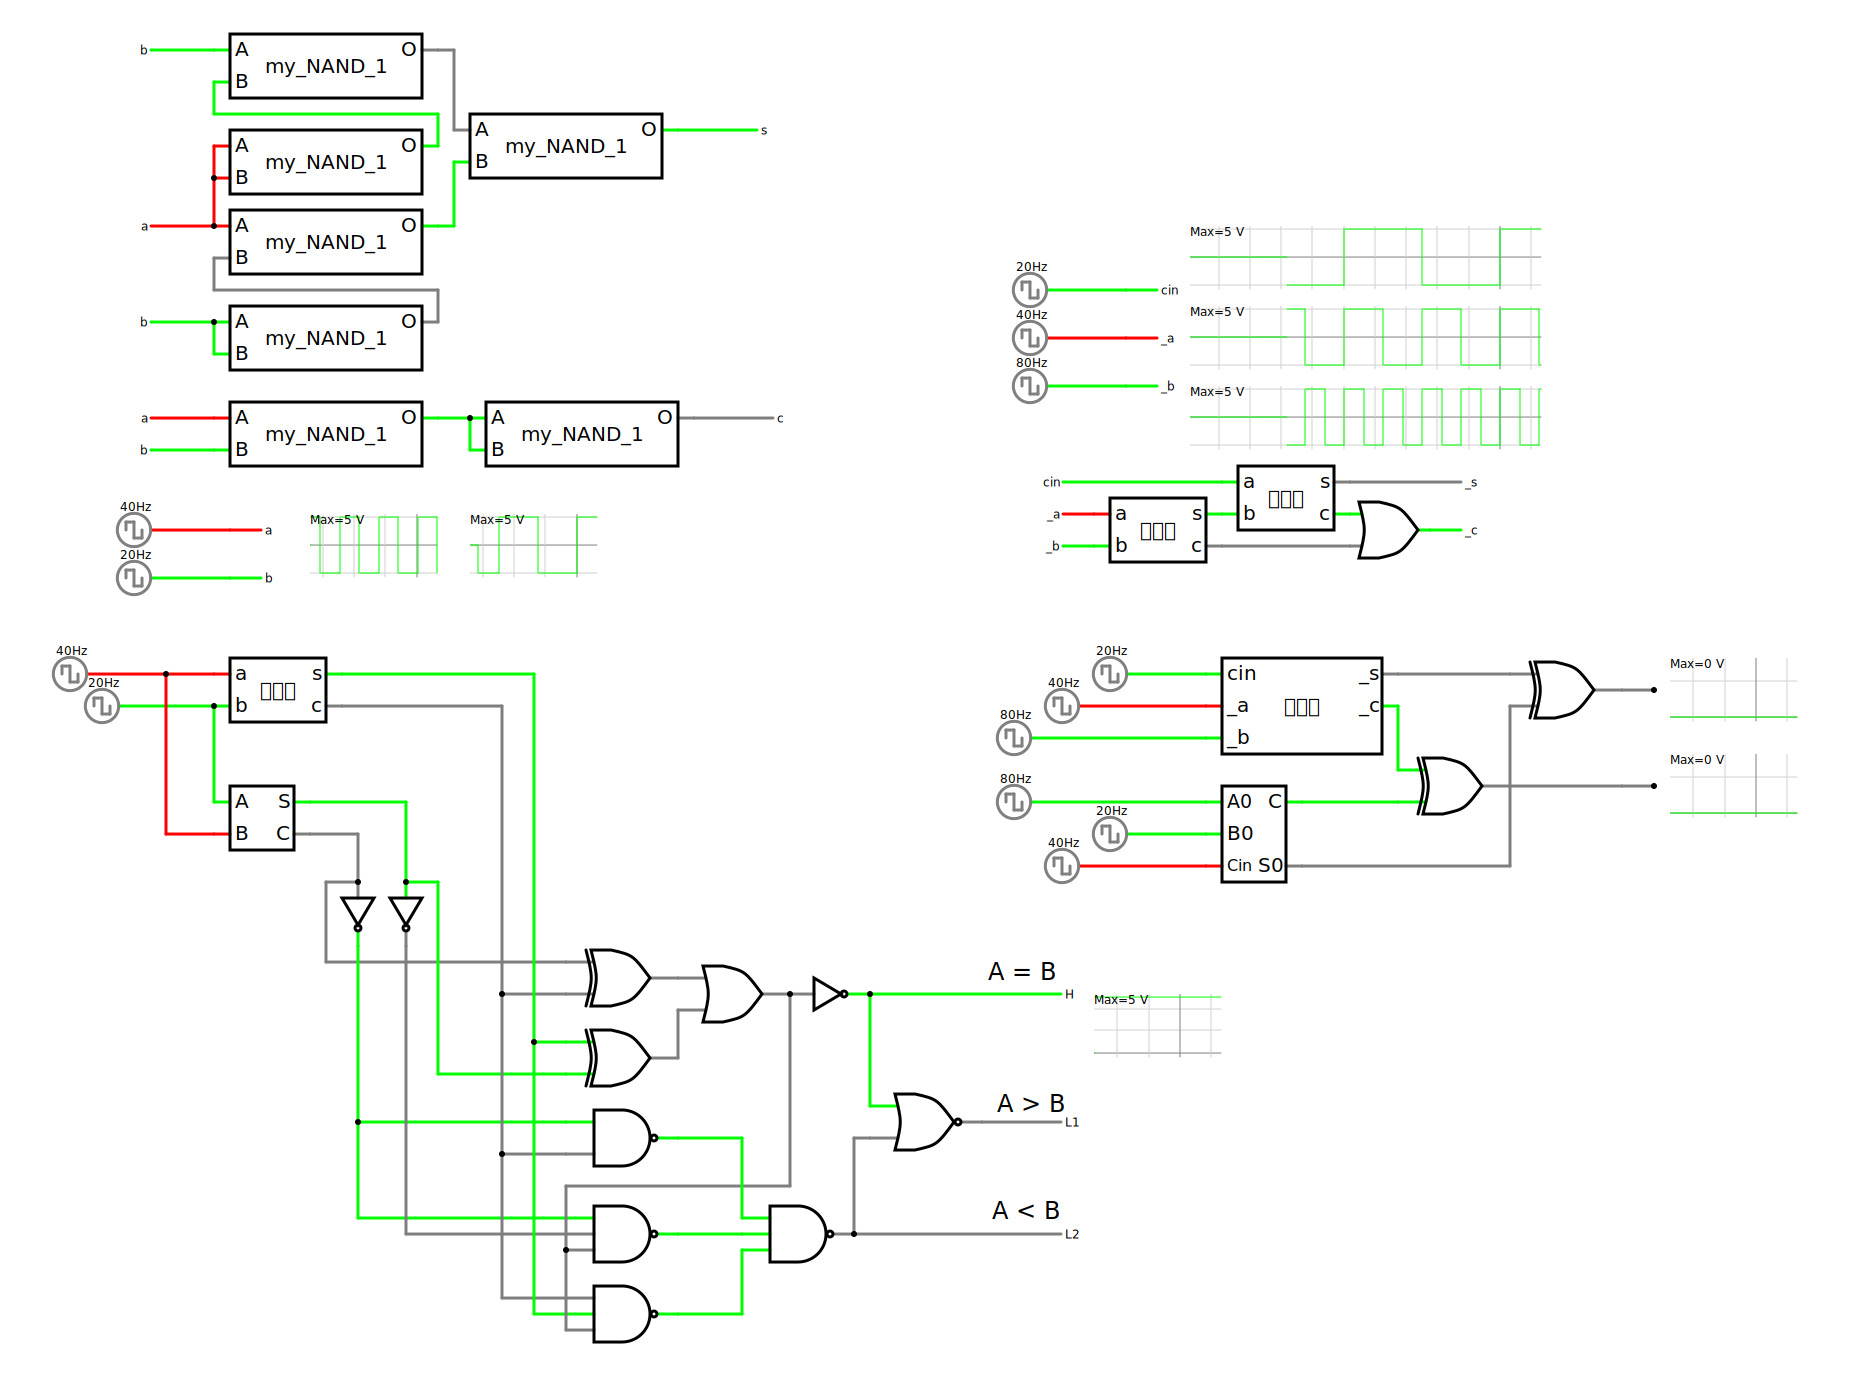
\includegraphics[width=1\textwidth]{半加器与全加器.pdf}
    \caption{半加器与全加器构建}
    \label{fig:banjiaqiyuquanjiaqi}
\end{figure}

\section{4-bit 乘法器}

乘法器的逻辑实现如图\ref{fig:chengfaqishixian} \np

\begin{figure}[htbp]
    \centering
    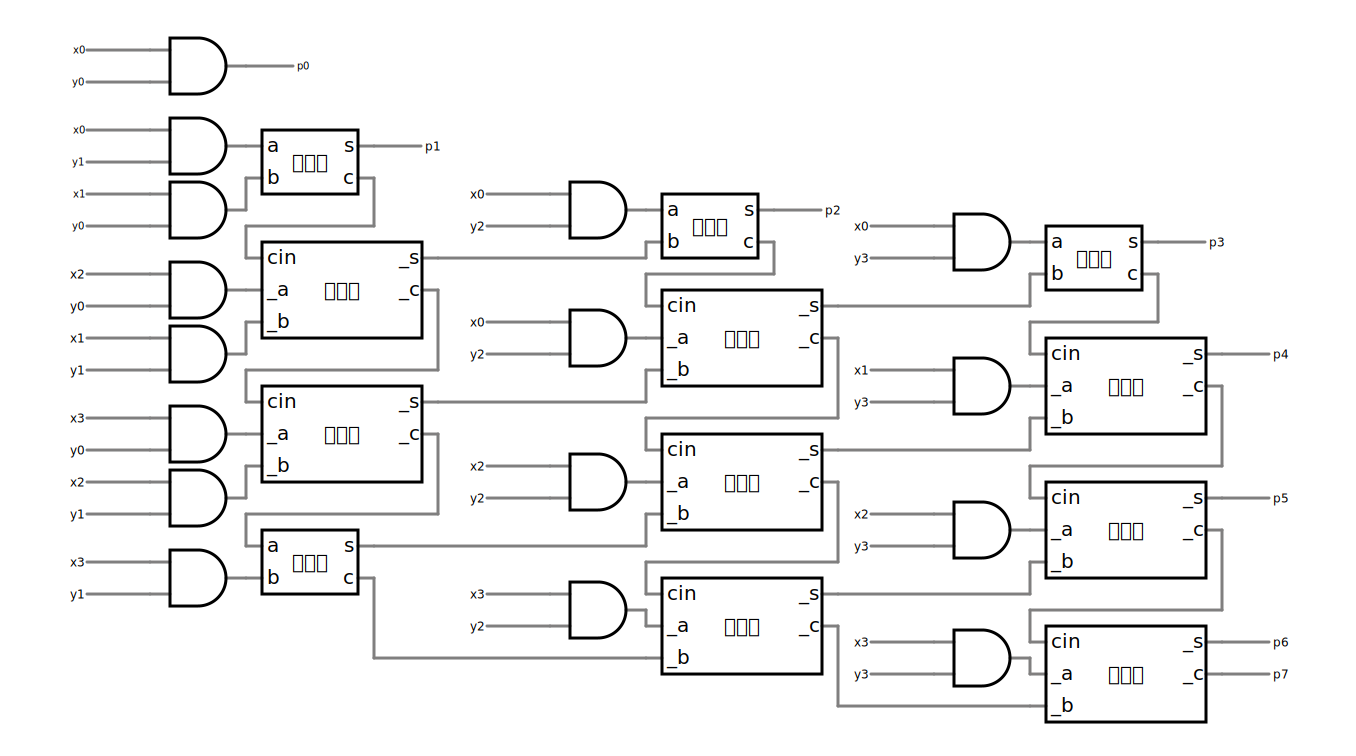
\includegraphics[width=1\textwidth]{4-bit乘法器.pdf}
    \caption{乘法器实现}
    \label{fig:chengfaqishixian}
\end{figure}

乘法器的文件验证图\ref{fig:chengfaqiyanzheng}

\begin{figure}[htbp]
    \centering
    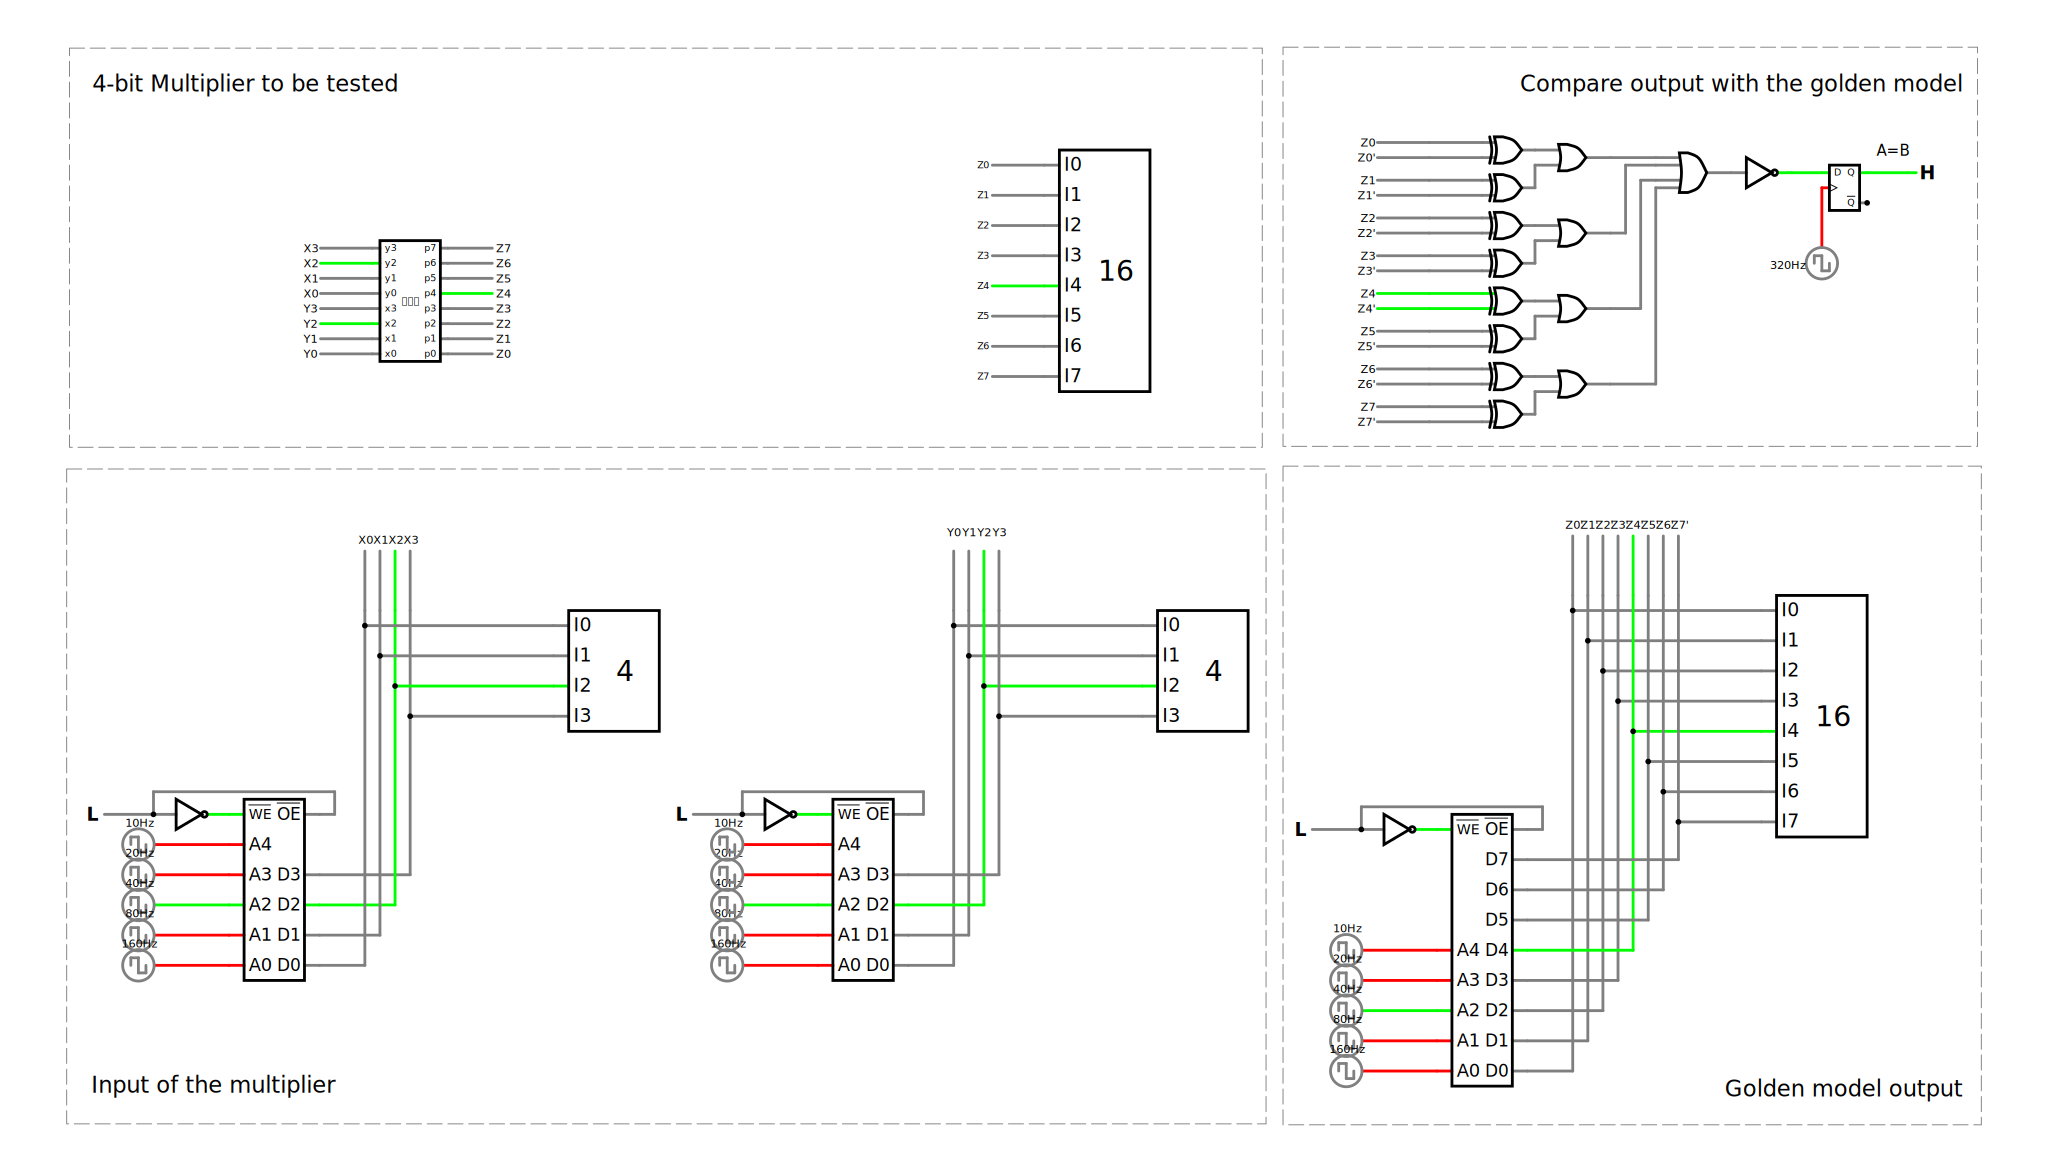
\includegraphics[width=1\textwidth]{乘法器验证.pdf}
    \caption{乘法器验证}
    \label{fig:chengfaqiyanzheng}
\end{figure}

\end{document}